
\newcommand{\LPprob}{\prob{Linear Programming}\xspace}
\newcommand{\IntLP}{\prob{Integer Linear Programming}}
\newcommand{\defn}[1]{\emph{#1}}

\section{Linear Programming and Integer Linear Programming}\label{flow: sec: LP}\doHeader{Linear Programming}

Recall that linear algebra is the study of systems of linear equations,
which are useful for modeling a wide variety of problems.
\emph{Linear programming} can be understood as a generalization of linear algebra,
in that it is about systems of linear \emph{inequalities} (including equations).
Linear \emph{inequalities} allow us to model an even wider variety of problems.

As a computational problem, an instance of \LPprob\ requires finding a vector 
that optimizes a given linear objective function subject to given linear constraints.
For example, given a matrix $A\in \R^{n\times m}$ and vectors $b\in \R^n$, $c\in \R^m$, 
find
\[ \min \{ c\cdot x ~|~ x\in \R^m;~x\ge 0; ~Ax \ge b\}.\]
A vector inequality such as $x \ge 0$ is interpreted component-wise,
% [review 2026-09-27] fix: x has m entries (n is the number of rows of A), so the index range is 1..m
i.e., as $x_i \ge 0$ for all $i\in\{1,2,\ldots,m\}$.
Similarly, $Ax \ge b$ is interpreted component-wise.

A \defn{feasible solution}
is any vector $x$ satisfying the constraints $x\in\R^m$, $x\ge 0$, and $Ax \ge b$.
The objective function (or \emph{cost}) is $c\cdot x = \sum_j c_j x_j$.
Linear programs may take other forms, for example
\( \max \{ c\cdot x ~|~ x\in \R^m;~x\ge 0; ~Ax \le b\}\).

\paragraph{\prob{Integer Linear Programming}.}
\emph{Integer Linear Programming} extends \LPprob by allowing an additional constraint
on the solution, namely, that each variable should be assigned an \emph{integer} value.
For example, given $(A,b,c)$ as above, find
\( \min \{ c\cdot x ~|~ x\in \Z^m;~x\ge 0; ~Ax \ge b\}\).
(Note that $\Z^m$ is the set of $m$-dimensional integer vectors.)
% A linear program (or integer linear program) 
% is a \defn{packing} problem provided 
% it is of the form $\max \{c\cdot x ~|~ A x \le b, x \ge 0\}$
% where every entry in $A$ is non-negative.
% Likewise, a linear program is a \defn{covering} problem if
% it is of the form $\min \{c\cdot x ~|~ A x \ge b, x \ge 0\}$,
% and $A$ has only non-negative entries.
\IntLP\ is a so-called \emph{NP-hard} problem---it is powerful enough to model many computationally \emph{intractable} combinatorial problems.
So \IntLP\ is unlikely to have a polynomial-time algorithm.
Nonetheless, many moderately sized Integer Linear Programs can be solved in practice,
so formulating a problem as an integer linear program can be an effective way to solve it.

\paragraph{A small linear program.}

\begin{figure}\centering
{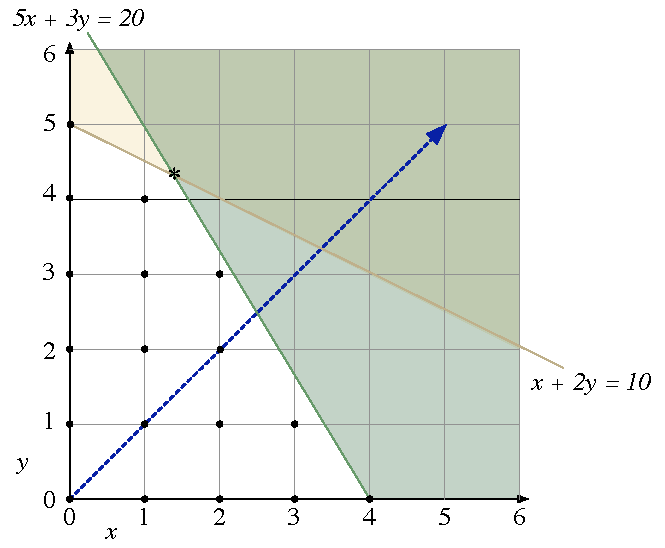
\includegraphics[width=3in]{31_linear_program}}
\caption{The two-dimensional linear program $\max\{ x + y : x, y\ge 0; x + 2y \le 10; 5x+3y \le 20\}$.
The feasible region is the white portion of the positive quadrant.
The optimal point is marked with an asterisk.}\label{flow: fig: LP}
\end{figure}

Consider the problem $\textsf{maximize } x+y$ subject to
$x+2y\le 10$,
$5x+3y \le 20$,
and $x,y\ge 0$.
The problem is illustrated in Figure~\ref{flow: fig: LP}.
The feasible region is the white area in the positive quadrant.
The dashed vector points in the direction of increasing cost ($x+y$).
The optimal feasible solution is $(1\frac{3}{7},4\frac{2}{7})$ (marked by ``*''),
of cost $5\frac{5}{7}$.
The feasible integer solutions 
(feasible solutions of the corresponding integer linear program)
are marked with black dots.
Three of these have maximum cost $5$.
The solution $(2,2)$ of cost $4$
is a $1\frac{1}{4}$-approximate solution to the integer linear program
and a $1\frac{3}{7}$-approximate solution to the linear program.

\paragraph{Algorithms for \prob{Linear Programming}.}
\LPprob\ is efficiently solvable.
That is, there are poly\-no\-mial-time algorithms that,
given any linear program, find an optimal solution.
Historically the so-called \emph{Simplex algorithm} is the most common.
Its worst-case run time is not polynomial, but it usually works quickly in practice.
In recent decades \emph{Interior-point} algorithms have superseded the Simplex algorithm.
These are polynomial-time algorithms.
The \emph{Ellipsoid} algorithm was the first polynomial-time algorithm to be discovered,
but it is slow in practice, so is of mostly theoretical interest.

\paragraph{Algorithms via \prob{Linear Programming}.}
Here's one technique for solving a given computational problem:
\begin{enumerate}[label=(\roman*)]
\item Model the problem as a linear program, that is, reduce the problem to \prob{Linear Programming}.
\item Use an existing LP solver to solve the linear program, and, therefore, your problem.
\end{enumerate}
This approach can be easier than designing an algorithm from scratch.
In the rest of this section we describe how various problems reduce to \prob{Linear Programming}.

\smallskip

We note in passing that there is another, more sophisticated, approach:
\begin{enumerate}[label=(\roman*)]
\item Model the problem as a linear program.
\item Design an efficient algorithm that mimics what the Simplex algorithm does for that linear program. 
\end{enumerate}
For example, the Ford-Fulkerson \prob{Max-Flow} algorithm
and Dijkstra's algorithm for \prob{Single-Source Shortest Paths}
% [review 2026-09-27] fix: "are special cases of Simplex" overstated an informal correspondence
can be viewed as special cases of the Simplex algorithm,
obtained by applying the Simplex algorithm (with suitable choices of pivots) to the linear programs for those problems.
We won't discuss this further here, as we don't discuss how the Simplex algorithm works.
Chapter 7 of \DPV discusses this approach specifically for \prob{Max Flow}.

\subsection{Max Flow as a linear program}  
Linear programs are often given by explicitly writing the constraints, rather than using a matrix.
For example, a given \prob{Max Flow} instance $(G=(V, E), s, t)$ translates directly to the following linear program: 
\[
\begin{LP}{~~\text{maximize~~}\sum_{w \in \out s} f_{sw} \,-\, \sum_{u \in \into s} f_{us}
    \text{~~~subject to:}}
  \big(\forall (u,w)\in E\big) && 0 ~\le~ f_{uw} & ~\le~ \capOf {u,w}
  && \comment{--- capacity constraints} \\[10pt]
  \big(\forall v\in V\setminus\{s,t\}\big)
  && \sum_{w\in \out v} f_{vw}
                                   & ~= \sum_{u\in \into v} f_{uv}
  && \comment{--- conservation constraints}
\end{LP}
\]
This is a (very easy!) polynomial-time reduction from \prob{Max Flow} to \LPprob.

Recall that, if the edge capacities are integers, then there is always an optimal integer-valued flow.
So, in this case, this linear program always has an optimal integer solution,
and finding one is not hard.

Recall that \prob{Bipartite Matching} and \prob{Disjoint Paths} reduce in polynomial time
to \prob{Max Flow}.
Since \prob{Max Flow} reduces to \LPprob, it follows that
these two problems also reduce to \LPprob.
As an exercise, you could try formulating each of these problems as a linear program directly.


\subsection{Min Cut as a linear program} 
A given \prob{Min Cut} instance $(G=(V, E), s, t)$ is equivalent to the following linear program: 

\[
\begin{LP}{~~\text{minimize~~}\sum_{(u, w)\in E} \capOf {u, w}\, x_{uw} \text{~~~subject to:}}
  && y_s &{} = 0; y_t {} = 1 \\
  \big(\forall v\in V\big) && 0 &{} \le y_v \le 1 \\
  \big(\forall (u, w)\in E\big) && 0 &{}\le x_{uw} \\
  % [review 2026-09-27] fix: y_v (v unbound) should be y_u, the tail of the edge (as the proof of the rounding lemma below uses)
  \big(\forall (u, w)\in E\big) && y_w - y_u & {} \le x_{uw}
\end{LP}
\]

The next lemma summarizes the relation to \prob{Min Cut}:
% [review 2026-09-27] fix: the lemma claimed a bijection between cuts and integer solutions with equal cost/capacity; but any integer x with x_uw >= max(0, y_w - y_u) is feasible, so a cut corresponds to many integer solutions, most costing more than the cut; restated as the two inequalities that the rounding lemma below actually uses
\begin{lemma}\label{flow: lemma: min cut LP}
  For any \prob{Min Cut} instance,
  every $s$-$t$ cut $(S, T)$ yields an integer solution to this linear program
  whose cost $\sum_{(u,w)\in E} \capOf{u,w} x_{uw}$ equals $\capOf{S, T}$,
  and every integer solution yields an $s$-$t$ cut
  whose capacity is at most the cost of the solution.
  In particular, the minimum cost of any integer solution is the minimum capacity of any $s$-$t$ cut.
\end{lemma}
\begin{proof}[Proof sketch.]
  Given any $s$-$t$ cut $(S, T)$,
  the corresponding (integer) solution $(x, y)$ to the linear program is obtained by taking
  \(y_v = 0\) for $v\in S$ and \(y_v=1\) for $v\in T$,
  and then $x_{uw} = 1$ for each edge $(u, w)$ that crosses the cut,
  and $x_{uw} = 0$ for each edge that doesn't cross the cut.
  One can verify that this must be a feasible solution with the correct cost.
  Conversely, given any integer solution $(x, y)$ to the linear program,
  the corresponding $s$-$t$ cut $(S, T)$ is obtained by taking $S=\{v \in V : y_v = 0\}$
  and $T=\{v\in V: y_v = 1\} = V\setminus S$.
  % [review 2026-09-27] fix: the capacity is at most the cost, not equal to it (each edge crossing the cut has y_w - y_u = 1, so x_uw >= 1, while other edges may also have x_uw > 0)
  This is an $s$-$t$ cut, and its capacity is at most the cost of $(x, y)$:
  each edge $(u, w)$ that crosses the cut has $y_w - y_u = 1$, so $x_{uw} \ge 1$.
\end{proof}

\providecommand{\wikipedia}[2]{\href{https://en.wikipedia.org/wiki/#2}{#1}}

Also, there is always an optimal integer solution to this linear program:
\begin{lemma}
  For any \prob{Min Cut} instance,
  there is an optimal integer solution to this linear program.
\end{lemma}
\begin{proof}
  Here's a clever proof using \wikipedia{the probabilistic method}{probabilistic method}.\footnote
  {If you're not familiar with probability, this proof won't make much sense.}
  Fix an instance and any optimal LP solution $(x, y)$.
  Choose a number $r\in [0,1]$ uniformly at random,
  then let
  \[S=\{v\in V : y_v \le r\} \text{ and } T=\{v \in V: y_v > r\}.\]
  This gives a random $s$-$t$ cut $(S, T)$.
  By \wikipedia{linearity of expectation}{Expected_value\#Basic_properties}, the expected capacity of this cut is
  \begin{align*}
    \sum_{(u, w)\in E} \capOf{u,w} \Pr[(u,w) \text{ crosses the cut}]
    & {} =
      \sum_{(u, w)\in E} \capOf{u,w} \Pr[ y_u \le r < y_w] &&(\comment{by definition of } (S, T)) \\
    & {} =
      \sum_{(u, w)\in E} \capOf{u,w} \max(0, y_w - y_u) && (\comment{by definition of } r)\\
    & {} \le
      \sum_{(u, w)\in E} \capOf{u,w} x_{uw} && (\comment{by inspection of the LP})
  \end{align*}
  That is, the expected capacity of the random cut $(S, T)$ is at most the cost of $(x, y)$.
  Thus, there must \emph{exist} a cut $(S^*, T^*)$ whose capacity is at most the cost of $(x, y)$.
  By Lemma~\ref{flow: lemma: min cut LP}, this cut $(S^*, T^*)$ has a corresponding integer solution $(x^*, y^*)$
  whose cost equals the capacity of $(S^*, T^*)$, which is in turn at most the cost of $(x, y)$.
  So $(x^*, y^*)$ is also optimal.
\end{proof}
\providecommand{\inbrs}{\text{\sf in}} 
\providecommand{\onbrs}{\text{\sf out}} 

\subsection{Shortest $s$-$t$ path as a linear program}\label{flow: sec: shortest path as LP}
Given a directed graph $G=(V, E)$ with non-negative edge weights,
and two vertices $s$ and $t$,
consider problem of finding a shortest path from $s$ to $t$ in $G$.
Here are two linear programs that model this problem.
We call one the \emph{primal} and the other the \emph{dual}:\footnote
{The existence of two such linear programs for a problem is not a coincidence.
  It happens for every linear-programming problem!
  The Max-Flow/Min-Cut relationship is another example.}

\begin{equation*}
  \begin{array}{c|c}
    \text{\emph{primal}} & \text{\emph{dual}}\\
    \begin{LP}{\text{minimize } \sum_{(u,w)\in E} \weight {u,w}\,f_{uw} \text{~~~subject to}}
      & (\forall v\in V) 
      & \sum_{w\in \onbrs(v)} f_{vw} - \sum_{w\in \inbrs(v)} f_{wv} 
      & =\,
      \begin{cases}
        1 & \text{ if } v=s \\
        -1 & \text{ if } v=t \\
        0 & \text{ otherwise}
      \end{cases}
      % [review 2026-09-27] fix: the non-negativity constraints were missing (without them the LP is unbounded when G has a positive-weight cycle, and the dual shown is not its dual)
      \\ & (\forall (u,w)\in E) & f_{uw} & \ge\, 0
    \end{LP}
      &
        \begin{LP}{\text{maximize } \pi_t - \pi_s \text{~~subject to}}
          \\
          & (\forall (u,w)\in E) &~  \pi_w - \pi_u  & \le  \, \weight {u,w}
        \end{LP}
  \end{array}
\end{equation*}

For intuition, note that, in the primal linear program, $f$ is a flow of value 1 from $s$ to $t$.
Integer flows of this kind correspond to $s$-$t$ paths:
% [review 2026-09-27] fix: the lemma claimed a bijection between s-t paths and integer solutions; but an integer solution may also carry flow around a cycle, so it need not be a path; restated as the two inequalities that the next lemma actually uses
\begin{lemma}\label{flow: lemma: sp primal}
  Every $s$-$t$ path $P$ in $G$ yields an integer solution $f$ to the primal whose cost is $\weight P$,
  and every integer solution $f$ yields an $s$-$t$ path whose weight is at most the cost of $f$.
  In particular, the minimum cost of any integer solution is $\dist s t$.
\end{lemma}
\begin{proof}[Proof sketch.]
  For any $s$-$t$ path $P$, the corresponding solution $f$ is defined by giving $f_{uw}$ a value equal to the number of times edge $(u, w)$ occurs in $P$.  Because the path starts at $s$, ends at $t$, and enters each other vertex $v$ the same number of times it leaves $v$, this assignment to $f$ meets the constraints of the primal LP.
  By inspection the cost of $f$ in the LP equals $\weight P$.

  Conversely, given any integer solution $f$ to the LP, one can construct a corresponding path $P$ by starting at $s$,
  then walking greedily, taking each step along any edge $(u, w)$ where $f_{uw}$ is positive.  When traversing an edge $(u, w)$,
  append the edge to $P$ and decrement $f_{uw}$.  Because $f$ satisfies the LP constraints,
  a greedy step is always possible until the walk reaches $t$.
  % [review 2026-09-27] fix: the walk may repeat vertices; since the weights are non-negative it contains an s-t path of no greater weight (this is what the lemma now claims)
  At that point $P$ is an $s$-$t$ walk of weight at most the cost of $f$ (the flow left over on edges of $f$ costs at least 0),
  and, because the edge weights are non-negative, $P$ contains an $s$-$t$ path of weight at most $\weight P$.
\end{proof}

\begin{lemma}
  The primal LP always has an optimal integer solution.
\end{lemma}
\begin{proof}[Proof sketch.]
  By an argument similar to the greedy construction in the previous proof, one can show that any solution $f$
  can be expressed as a weighted average of some integer solutions $f_1, f_2, \ldots, f_\ell$.
  The cost of $f$ equals the average cost of these solutions,
  so the cheapeast of these integer solutions has cost at most the cost of $f$.
\end{proof}

It follows that the value of the linear program (that is, the optimal objective value achieved by any feasible solution)
is $\dist s t$.
Next we consider the dual LP, and show the same for it:

\begin{lemma}\label{flow: lemma: dual LP value}
  The value of the dual LP is $\dist s t$.
\end{lemma}
\begin{proof}
  First we show that the value of the dual LP is at most $\dist s t$.
  Let $\pi^*$ be an optimal solution to the dual LP, so $\pi^*_t - \pi^*_s$ is the value of the dual LP.
  Let $P^*$ be a shortest $s$-$t$ path, so $\weight {P^*} = \dist s t$.
  Then, summing the dual LP constraints over edges in $P^*$ gives
  \[
    \dist s t
    = \weight {P^*}
    = \sum_{(u,w)\in P^*} \weight {u, w}
    \ge \sum_{(u,w)\in P^*} \pi^*_w - \pi^*_u
    % [review 2026-09-27] fix: the telescoping sum equals pi_t - pi_s (it was written as pi_s - pi_t, the negative of the dual objective)
    ~=~ \pi^*_t - \pi^*_s.
  \]
  The last step follows because the sum ``telescopes''---for each vertex $v$ on the interior of the path $P^*$,
  the term $\pi^*_v$ occurs once with positive sign and once with negative sign,
  and these terms cancel each other.

  To finish we show that the value of the dual LP is at least $\dist s t$.
  % [review 2026-09-27] fix: dist(s,v) is infinite for vertices not reachable from s; they can be discarded first
  Define a dual solution $\pi$ by taking $\pi_v = \dist s v$ for every $v$
  (assuming every vertex is reachable from $s$; deleting the unreachable vertices changes neither $\dist s t$ nor the LPs' values).
  This solution $\pi$ is feasible, because by the triangle inequality,\footnote
  {The triangle inequality is that $\dist s w \le \dist s u + \weight {u, w}$.
    It holds because one way to get from $s$ to $w$ is to take a shortest path from $s$ to $u$,
    followed by the edge $(u, w)$.}
  for any edge $(u, w)$,
  \[
    \pi_w - \pi_u = \dist s w - \dist s u \le \weight {u, w}.
  \]
  
  And the cost of $\pi$ is $\pi_t - \pi_s = \dist s t - \dist s s = \dist s t$. 
  So, the dual LP has a feasible solution of cost $\dist s t$,
  and is a maximization problem, so its value must be at least $\dist s t$.
\end{proof}

\subsection{Subset Sum as an integer linear program}
For variety, consider the \prob{Smallest Subset Sum} problem.
Fix an instance $(v=(v_1, v_2, \ldots, v_n), T)$.
The problem is to determine the smallest subsequence of $v$ that sums to $T$.
Here is an equivalent instance of Integer Linear Programming:
\[
\begin{LP}{~~\text{minimize~~}\textstyle\sum_{i=1}^n x_i
    \text{~~~subject to:}}
  \big(\forall i\in\{1,\ldots,n\}\big) && 0 \le x_i & {} \le 1, \\
  && \textstyle \sum_{i=1}^n v_i\, x_i & {} = T, \\
  && x & {} \in \Z^n.
\end{LP}
\]
Setting $x_i=1$ corresponds to including $v_i$ in the subsequence.
(And setting $x_i=0$ corresponds to omitting it.)
In this way, the solutions to this integer linear program
correspond bijectively to the subsequences of $v$ that sum to $T$.
The size of each subsequence equals the cost, $\sum_i x_i$, of its corresponding solution $x$.

What would happen if we were to drop the explicit integrality constraint, `` $x\in \Z^n$ ''?
This would give a linear program instead of an integer linear program.
But that linear program wouldn't necessarily have optimal solutions that are integer valued.
Consider for example the \prob{Smallest Subset Sum} instance $(v=(1,3), T=2)$.
It has no solution---no subsequence of $v$ sums to 2.
But the corresponding linear program has many solutions, the optimum being $x=(0, 2/3)$.

\subsection{External sources on linear programming}

\providecommand{\wikipedia}[2]{\href{https://en.wikipedia.org/wiki/#2}{#1}}

\begin{itemize}
\item \DPV Chapter 7.  \KT Section 11.6 and \KWSlides.  \CLRS Chapter 29. MIT lecture video:

  {\small
\URLplain{https://ocw.mit.edu/courses/electrical-engineering-and-computer-science/6-046j-design-and-analysis-of-algorithms-spring-2015/lecture-videos/lecture-15-linear-programming-lp-reductions-simplex/}}
  
\item \JE notes: \url{https://jeffe.cs.illinois.edu/teaching/algorithms/notes/H-lp.pdf}

\item Microsoft Excel has a free add-on for solving LPs in a spreadsheet.  See e.g.
  
  {\small
    \URLplain{https://www.fm-magazine.com/issues/2019/feb/linear-programming-microsoft-excel.html}}

\item For more serious applications, Gurobi has a commercial LP solver, free for academic use, that you can install on your own computer.  It can also solve Integer Linear Programs of moderate size.  \url{https://gurobi.com}

\item Many other free LP solvers are available.

\end{itemize}

%%% Local Variables:
%%% mode: latex
%%% TeX-master: "flow_reductions_LP"
%%% End:
